%%%%%%%%%%%%%%%%%%%%%%%%%%%%%%%%%%%%%%%%%%%%%%%%%%
%%%%%%%%%%%%%%%%%%%%%%%%%%%%%%%%%%%%%%%%%%%%%%%%%%
%%
%% Based one the "beamer-greek-two" template provided
%% by the Laboratory of Computational Mathematics,
%% Mathematical Software and Digital Typography,
%% Department of Mathematics, University of the Aegean
%% (http://myria.math.aegean.gr/labs/dt/)
%%
%% Adapted by John Liaperdos, October-November 2014
%% (ioannis.liaperdos@gmail.com)
%%
%% Last update: 22/06/2017 (English Support)
%% Source: https://es.overleaf.com/latex/templates/thesis-presentation-template-beamer-english-version-dpt-of-computer-engineering-technological-educational-institute-of-peloponnese/vwhtyshhtqmg
%%%%%%%%%%%%%%%%%%%%%%%%%%%%%%%%%%%%%%%%%%%%%%%%%%
%%%%%%%%%%%%%%%%%%%%%%%%%%%%%%%%%%%%%%%%%%%%%%%%%%
%%
\PassOptionsToPackage{unicode}{hyperref}
\PassOptionsToPackage{naturalnames}{hyperref}
\documentclass{beamer}
\usepackage[T1]{fontenc}
\usepackage[spanish]{babel}
\usepackage[utf8]{inputenc}
\usepackage{multicol}
\usepackage{caption}
\usepackage{subfig}
\usepackage{tikz}

%%% FONT SELECTION %%%%%%%%%%%%%%%%%
%%% we choose a sans font %%%%%%%%%%
\usepackage{kmath,kerkis}
%\usepackage[default]{gfsneohellenic}
%%%%%%%%%%%%%%%%%%%%%%%%%%%%%%%%%%%%

\usepackage{color}
\usepackage{amsmath}
\usepackage{amssymb}
\usepackage{xcolor}

% Syntax: \colorboxed[<color model>]{<color specification>}{<math formula>}
\newcommand*{\colorboxed}{}
\def\colorboxed#1#{%
  \colorboxedAux{#1}%
}
\newcommand*{\colorboxedAux}[3]{%
  % #1: optional argument for color model
  % #2: color specification
  % #3: formula
  \begingroup
    \colorlet{cb@saved}{.}%
    \color#1{#2}%
    \boxed{%
      \color{cb@saved}%
      #3%
    }%
  \endgroup
}
\usepackage{epstopdf}
\usepackage{graphicx}
\graphicspath{{./img/}}

%%
% load TEI-Pel - specific layout
\usepackage{TeiPel_En_Beamer_Layout}
\setTeipelLayout{draft,newlogo}% options: "draft", "newlogo"

%%%%%%%%%%%%%%%%%%%%%%%%%%%%%%%%%%%%%%%%%%%%%%%%%%%%%%%%%%%%
% Thesis Info %%%%%%%%%%%%%%%%%%%%%%%%%%%%%%%%%%%%%%%%%%%%%%
%%%%%%%%%%%%%%%%%%%%%%%%%%%%%%%%%%%%%%%%%%%%%%%%%%%%%%%%%%%%
	% title
		\title[Any2Vec - Embeddings para búsqueda de semántica y aritmética de contenidos no verbales]{Any2Vec - Embeddings para búsqueda de semántica y aritmética de contenidos no verbales}
	% author
    % (In the mandatory argument "{}", separate multiple
    % authors with "\and" - use "\\" for better author name formatting
    % in the title page. In the optional argument "[]" include all
	% author names, with no "\and" or text formatting macros.)
	% Example:
    %\author[A. Author Albert Einstein]{Anthony Author \and Albert Einstein}
		\author[A. Gámiz]{Antonio Gámiz Delgado}
	% supervisor
		% \supervisor{Supervisor}{Mister Supervisor}{Professor}
	% date
		\presentationDate{? de noviembre de 2022}
%%%%%%%%%%%%%%%%

\begin{document}

% typeset front slides
	\typesetFrontSlides

%%%%%%%%%%%%%%%%
% Your Slides Start here:

%%%%
\section{Introducción}

\subsection[Problema]{Descripción del problema}

\begin{frame}{Motivación}
  \framesubtitle{Desarrollo de narrativas}
	\begin{itemize}
    \item ¿Qué conjunto de tropos funcionan bien juntos?
    \item ¿Hay conjuntos de tropos que no casen bien?
    \item ¿Qué combinación de tropos puedo usar para aumentar la probabilidad de éxito de mi película?
    \item Aritmética de tropos
  \end{itemize}
\end{frame}

\begin{frame}{Descripción}
  \begin{itemize}
    \item Crear un modelo para que otros investigadores puedan analizar contenido no verbal.
    \item Analizar las relaciones entre los tropos de películas.
  \end{itemize}
\end{frame}

\begin{frame}{Metodología}
	\begin{itemize}
		\item Desarrollo ágil
		\item \textit{Test Driven Development (TDD)}
		\item \textit{Domain Driven Design (DDD)}
		\item Integración continua
	\end{itemize}
\end{frame}

\section{Word2Vec}

\begin{frame}{Word2Vec}
	\begin{figure}[ht]
		\centering
		\begin{tikzpicture}[
						roundnode/.style={circle, draw=black, minimum size=5mm},
				]

				\node[roundnode]   at (5,5)   (rey)  {\tiny Rey};
				\node[roundnode]   at (4,4)   (hombre)  {\tiny Hombre};
				\node[roundnode]   at (6,4)   (reina)  {\tiny Reina};
				\node[roundnode]   at (5,3)   (mujer)  {\tiny Mujer};

				\draw[-stealth] (rey) -- (reina);
				\draw[-stealth] (hombre) -- (mujer);

		\end{tikzpicture}
		\caption{Reina = Rey - Hombre + Mujer}
	\end{figure}
\end{frame}

\begin{frame}
	\begin{definition}
		Un vector \textit{one-hot encoded} es un vector donde solo una de sus componentes es 1.
	\end{definition}
	Dado un vocabulario con $n\in\mathbb{N}$ términos, habrá $n$ vectores diferentes donde el íncide
	que ocupa un término caracteriza a la palabra. Por ejemplo:
	\begin{equation}
		\text{Sea } w_j\in V, \text{ su vector sería } \{0, \cdots, \underbrace{1}_{j}, \cdots, 0\}
	\end{equation}

\end{frame}

\subsection{Bolsa continua de palabras}

\begin{frame}{Bolsa continua de palabras}
	\begin{figure}[ht]
		\centering
		\begin{tikzpicture}[
						roundnode/.style={circle, draw=black, minimum size=4mm},scale=0.75,every node/.style={scale=0.75}
				]

				\node[rectangle, draw, minimum width = 0.3cm, minimum height = 2cm] (xck) at (0.5,0) {};
				\node[] at (-0.2,0) {$x_{Ck}$};
				\draw[] (0.5, 0.7) circle (0.1cm);
				\draw[] (0.5, 0.3) circle (0.1cm);
				\draw[] (0.5, -0.7) circle (0.1cm);
				\path (0.5, -0.9) -- (0.5, 0.3) node [black, midway, sloped] {$\dots$};

				\node[rectangle, draw, minimum width = 0.3cm, minimum height = 2cm] (xdk) at (0.5,3) {};
				\node[] at (-0.2,3) {$x_{2k}$};
				\draw[] (0.5, 3.7) circle (0.1cm);
				\draw[] (0.5, 3.3) circle (0.1cm);
				\draw[] (0.5, 2.3) circle (0.1cm);
				\path (0.5, 2.3) -- (0.5, 3.3) node [black, midway, sloped] {$\dots$};

				\node[rectangle, draw, minimum width = 0.3cm, minimum height = 2cm] (xuk) at (0.5,6) {};
				\node[] at (-0.2,6) {$x_{1k}$};
				\draw[] (0.5, 6.7) circle (0.1cm);
				\draw[] (0.5, 6.3) circle (0.1cm);
				\draw[] (0.5, 5.3) circle (0.1cm);
				\path (0.5, 5.3) -- (0.5, 6.3) node [black, midway, sloped] {$\dots$};

				\path (xdk) -- (xck) node [black, midway, sloped] {$\dots$};

			 % ========= hidden layer


				\node[rectangle, draw, minimum width = 0.3cm, minimum height = 1.6cm] (xdk) at (3.5,3) {};
				\node[] at (4,3) {$h$};
				\draw[] (3.5, 3.5) circle (0.1cm);
				\draw[] (3.5, 2.4) circle (0.1cm);
				\path (3.5, 2.4) -- (3.5, 3.5) node [black, midway, sloped] {$\dots$};

			 % ========= connections input->hidden layer

			 \draw[] (0.65,1) -- (3.35,3.8);
			 \draw[] (0.65,4) -- (3.35,3.8);
			 \draw[] (0.65,7) -- (3.35,3.8);

			 \draw[] (0.65,-1) -- (3.35,2.2);
			 \draw[] (0.65,2) -- (3.35,2.2);
			 \draw[] (0.65,5) -- (3.35,2.2);

			 \node[] at (1.5,0.8) {$W_{V\times N}$};
			 \node[] at (1.5,3) {$W_{V\times N}$};
			 \node[] at (1.5,5.3) {$W_{V\times N}$};


			 % ========= output layer

			 \node[rectangle, draw, minimum width = 0.3cm, minimum height = 4cm] (xdk) at (6.5,3) {};
			 \node[] at (7,3) {$y$};
			 \draw[] (6.5, 4.8) circle (0.1cm);
			 \draw[] (6.5, 4.5) circle (0.1cm);
			 \draw[] (6.5, 4.2) circle (0.1cm);
			 \draw[] (6.5, 3.9) circle (0.1cm);
			 \draw[] (6.5, 3.6) circle (0.1cm);
			 \draw[] (6.5, 1.4) circle (0.1cm);
			 \path (6.5, 1.4) -- (6.5, 3.6) node [black, midway, sloped] {$\dots$};


			 % ========= connections hidden->output layer

			 \draw[] (3.65,3.8) -- (6.35, 5);
			 \draw[] (3.65,2.2) -- (6.35, 1);

			 \node[] at (5,3) {$W'_{N\times V}$};

		\end{tikzpicture}
		\caption{CBOW con C palabras por contexto}
	\end{figure}
\end{frame}

\subsection{Skip-Gram}

\begin{frame}{Skip-Gram}
	\begin{figure}[ht]
		\centering
		\begin{tikzpicture}[
						roundnode/.style={circle, draw=black, minimum size=4mm},scale=0.75,every node/.style={scale=0.75}
				]
				\node[rectangle, draw, minimum width = 0.3cm, minimum height = 2cm] (xk) at (0.5,3) {};
				\node[] at (-0.2,3) {$x_{k}$};
				\draw[] (0.5, 3.7) circle (0.1cm);
				\draw[] (0.5, 3.3) circle (0.1cm);
				\draw[] (0.5, 2.3) circle (0.1cm);
				\path (0.5, 2.3) -- (0.5, 3.3) node [black, midway, sloped] {$\dots$};

				\node[rectangle, draw, minimum width = 0.3cm, minimum height = 1.6cm] (xdk) at (3.5,3) {};
				\node[] at (4,3) {$h$};
				\draw[] (3.5, 3.5) circle (0.1cm);
				\draw[] (3.5, 2.4) circle (0.1cm);
				\path (3.5, 2.4) -- (3.5, 3.5) node [black, midway, sloped] {$\dots$};

			%  % ========= connections input->hidden layer

			 \draw[] (0.65,4) -- (3.35,3.8);
			 \draw[] (0.65,2) -- (3.35,2.2);

			 \node[] at (1.5,3) {$W_{V\times N}$};


			%  % ========= output layer

				\node[rectangle, draw, minimum width = 0.3cm, minimum height = 2cm] (ycj) at (6.5,0) {};
				\node[] at (7,0) {$y_{Cj}$};
				\draw[] (6.5, 0.7) circle (0.1cm);
				\draw[] (6.5, 0.3) circle (0.1cm);
				\draw[] (6.5, -0.7) circle (0.1cm);
				\path (6.5, -0.9) -- (6.5, 0.3) node [black, midway, sloped] {$\dots$};

			\node[rectangle, draw, minimum width = 0.3cm, minimum height = 2cm] (ydj) at (6.5,3) {};
			\node[] at (7,3) {$y_{2k}$};
			\draw[] (6.5, 3.7) circle (0.1cm);
			\draw[] (6.5, 3.3) circle (0.1cm);
			\draw[] (6.5, 2.3) circle (0.1cm);
			\path (6.5, 2.3) -- (6.5, 3.3) node [black, midway, sloped] {$\dots$};

			\node[rectangle, draw, minimum width = 0.3cm, minimum height = 2cm] (yuj) at (6.5,6) {};
			\node[] at (7,6) {$y_{1k}$};
			\draw[] (6.5, 6.7) circle (0.1cm);
			\draw[] (6.5, 6.3) circle (0.1cm);
			\draw[] (6.5, 5.3) circle (0.1cm);
			\path (6.5, 5.3) -- (6.5, 6.3) node [black, midway, sloped] {$\dots$};

			\path (ydj) -- (ycj) node [black, midway, sloped] {$\dots$};

			%  % ========= connections hidden->output layer

			 \draw[] (3.65,3.8) -- (6.35, 7);
			 \draw[] (3.65,2.2) -- (6.35, 5);

			 \draw[] (3.65,3.8) -- (6.35, 4);
			 \draw[] (3.65,2.2) -- (6.35, 2);

			 \draw[] (3.65,3.8) -- (6.35, 1);
			 \draw[] (3.65,2.2) -- (6.35, -1);

			 \node[] at (5.5,5) {$W'_{N\times V}$};
			 \node[] at (5.5,3) {$W'_{N\times V}$};
			 \node[] at (5.5,1) {$W'_{N\times V}$};

		\end{tikzpicture}
		\caption{Skip-gram con C palabras por contexto}
	\end{figure}
\end{frame}

\begin{frame}{Función de activación}
	\begin{equation*}
		p(w_j|w_I) = \frac{\exp(v^{'T}_{w_j}v_{w_I})}{\sum_{j'=1}^V\exp(v^{'}_{w_{j'}}v_{w_I})}
	\end{equation*}
	donde
	\begin{equation*}
		v_{w_I}=W^Tx=W^T_{k, \cdot}=h
	\end{equation*}
	\begin{equation*}
		v^{'}_{w_j}=W^{'}_{\cdot, j}
	\end{equation*}
\end{frame}

\begin{frame}{Función de pérdida}
	\begin{equation}
		\begin{split}
			E & = -\log p\left( w_O | w_{I,1}, \cdots, w_{I, C} \right) \\
				& = -v_{w_O}^{'T}h + \log\displaystyle\sum_{j'=1}^V\exp\left(v'_{w_j}\right) \\
				& = -v_{w_O}^{'T}h + \log\displaystyle\sum_{j'=1}^V\exp\left( v_{w_j}^{'T}h \right) \\
		\end{split}
	\end{equation}
\end{frame}

\subsection{Optimización}

\begin{frame}{Optimización}
	\begin{equation*}
		p(w_j|w_I) = \frac{\exp(v^{'T}_{w_j}v_{w_I})}{\colorboxed{red}{\sum_{j'=1}^V\exp(v^{'}_{w_{j'}}v_{w_I})}}
	\end{equation*}
\end{frame}

\begin{frame}{Softmax jerárquico}
	\begin{figure}[H]
		\centering
		\begin{tikzpicture}[
						roundnode/.style={circle, draw=black, minimum size=7mm},
				]

				\node[roundnode, fill=gray,label=above:{$n(w_2, 1)$}]   at (3.5,7)   (root)  {};
				\node[roundnode, fill=gray,label=above:{$n(w_2, 2)$}]   at (2,6)   (n1)  {};
				\node[roundnode, fill=gray]   at (5,6)   (n2)  {};

				\draw[-stealth] (root) -- node[above,xshift=1cm]   {} (n1);
				\draw[-stealth] (root) -- node[above,xshift=1cm]   {} (n2);


				\node[roundnode, fill=gray,label=above:{$n(w_2, 3)$}]   at (1,5)   (n3)  {};
				\draw[-stealth] (n1) -- node[above,xshift=1cm]   {} (n3);

				\node[roundnode, fill=gray]   at (6,5)   (n4)  {};
				\draw[-stealth] (n2) -- node[above,xshift=1cm]   {} (n4);

				\node[roundnode,label=below:{$w_1$}]   at (0,4)   (n5)  {};
				\node[roundnode,label=below:{$w_2$}]   at (2,4)   (n6)  {};
				\draw[-stealth] (n3) -- node[above,xshift=1cm]   {} (n5);
				\draw[-stealth] (n3) -- node[above,xshift=1cm]   {} (n6);

				\node[roundnode,label=below:{$w_3$}]   at (3,4)   (n7)  {};
				\draw[-stealth] (n1) -- node[above,xshift=1cm]   {} (n7);

				\node[roundnode,label=below:{$w_4$}]   at (4,4)   (n8)  {};
				\draw[-stealth] (n2) -- node[above,xshift=1cm]   {} (n8);

				\node[roundnode,label=below:{$w_{V-1}$}]   at (6,4)   (n9)  {};
				\node[roundnode,label=below:{$w_V$}]   at (7,4)   (n10)  {};
				\draw[-stealth] (n4) -- node[above,xshift=1cm]   {} (n9);
				\draw[-stealth] (n4) -- node[above,xshift=1cm]   {} (n10);

				\path (n8) -- (n9) node [black, font=\Huge, midway, sloped] {$\dots$};

		\end{tikzpicture}
		\caption{Ejemplo de árbol binario de Huffman (no se incluyen frecuencias).}
	\end{figure}
\end{frame}

\begin{frame}{Softmax jerárquico}
	\begin{equation}\label{eq:soft}
		p\left( w=w_O \right) = \prod_{j=1}^{L(w)-1}\sigma\left( \llbracket n(w, j+1)=ch(n(w,j))\rrbracket v^{'T}_{n(w,j)}h \right)
	\end{equation}
	donde
	\begin{equation}
		\llbracket x \rrbracket = \begin{cases}
			1 & \text{ si x es cierto} \\
			-1 & \text{ si x es falso}
		\end{cases}
	\end{equation}
\end{frame}

\section{Resultados}

\begin{frame}
	\begin{center}
		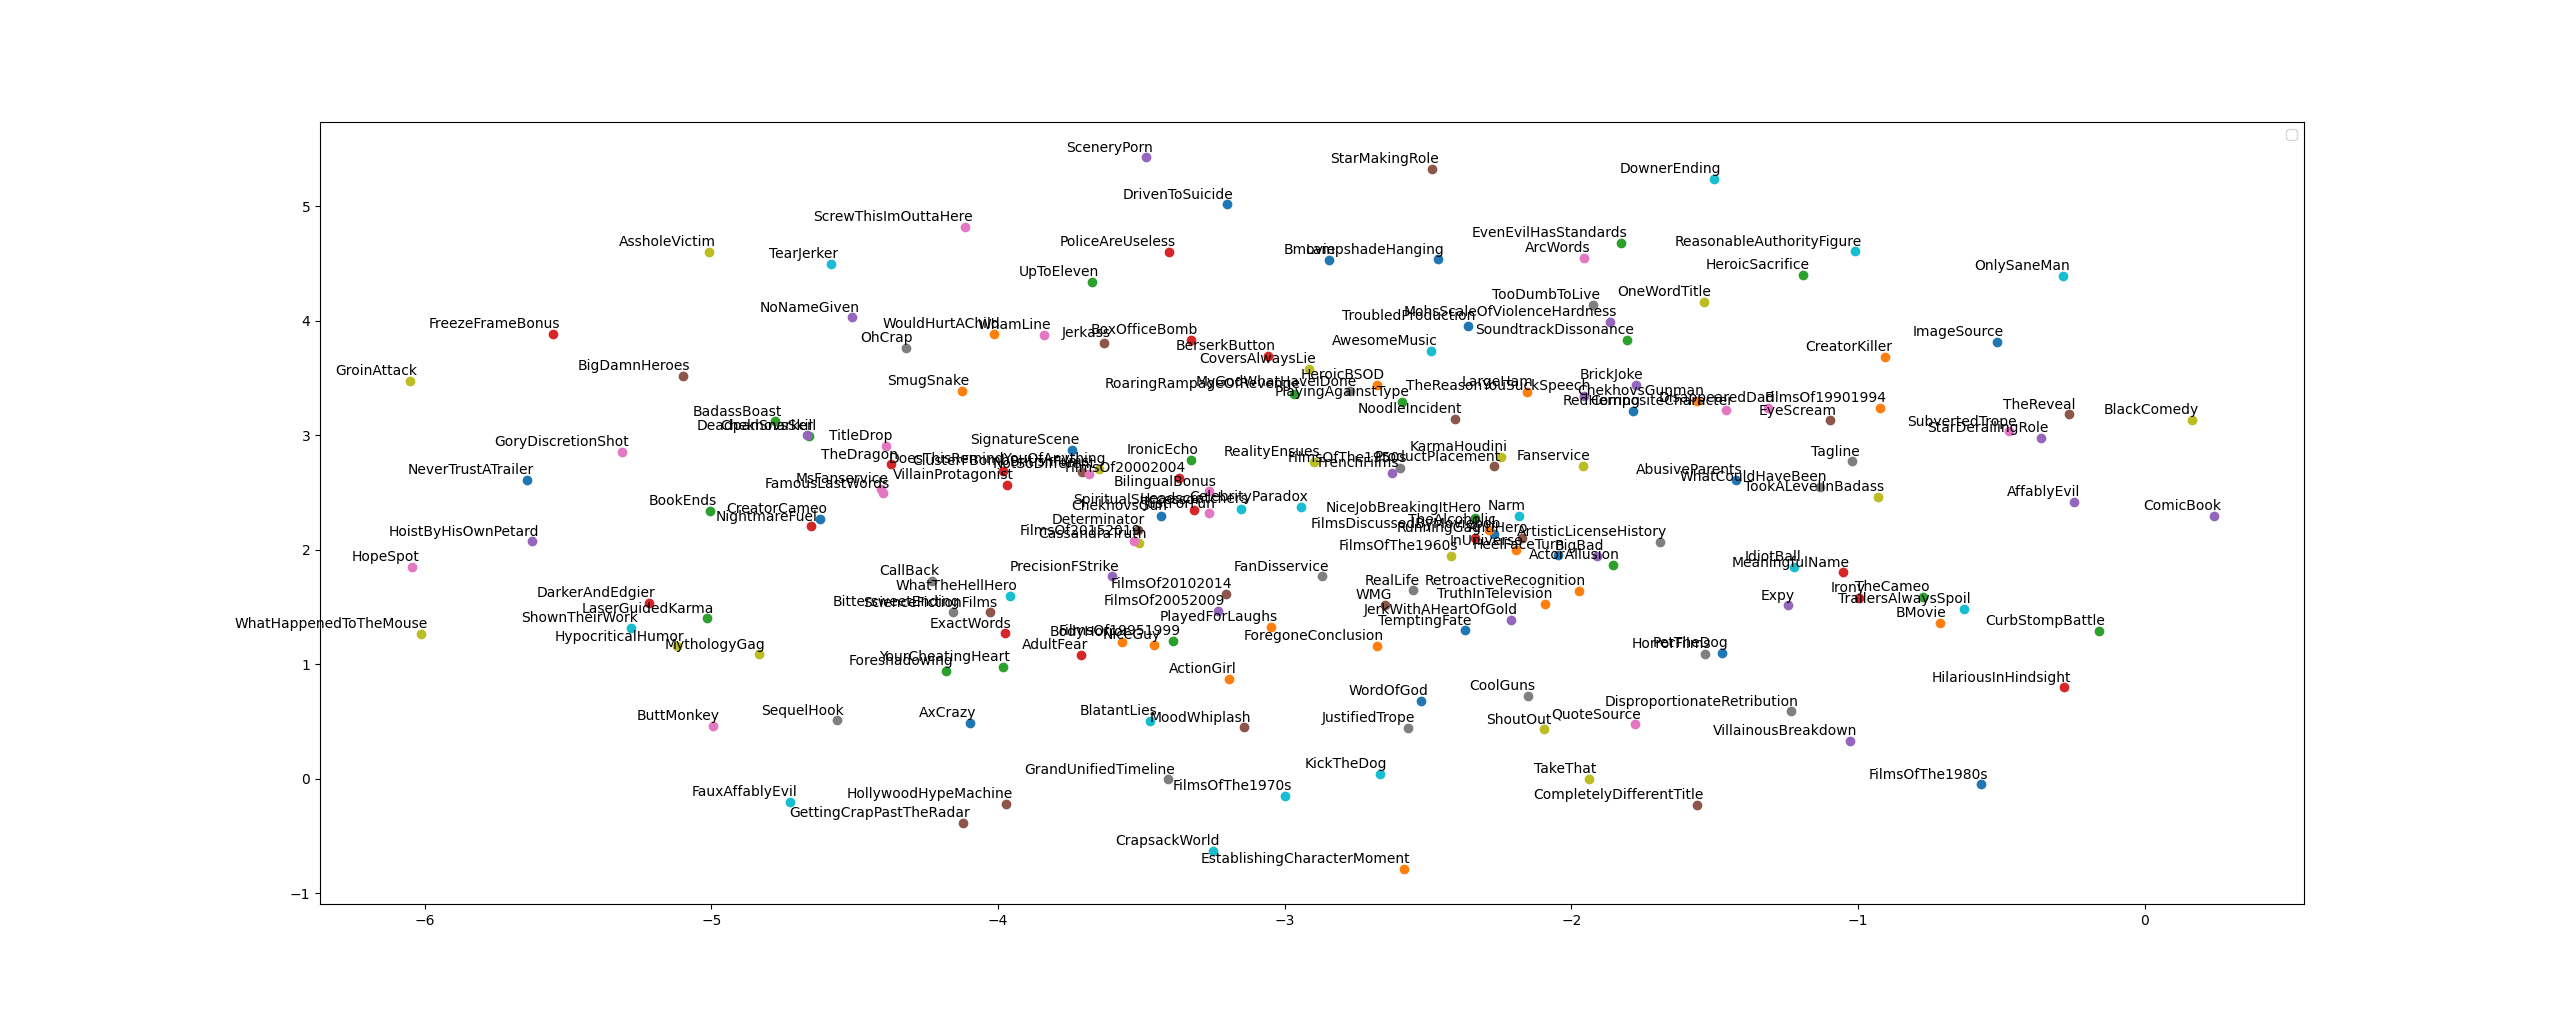
\includegraphics[width=0.95\textwidth,keepaspectratio]{tsne_full.png}
		\\
		\footnotesize(t-SNE)
    \end{center}
\end{frame}

\begin{frame}
	\begin{center}
		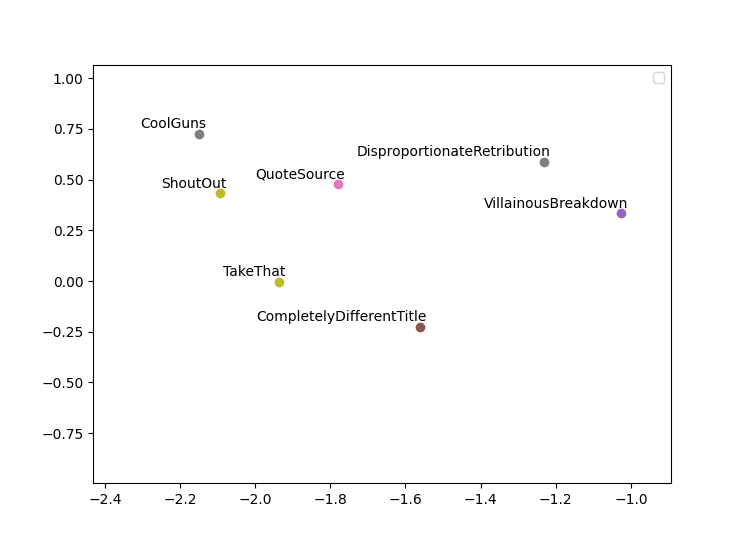
\includegraphics[width=0.85\textwidth,keepaspectratio]{tsne.png}
		\\
		\footnotesize(Ampliación t-SNE)
    \end{center}
\end{frame}

\begin{frame}
	\begin{center}
		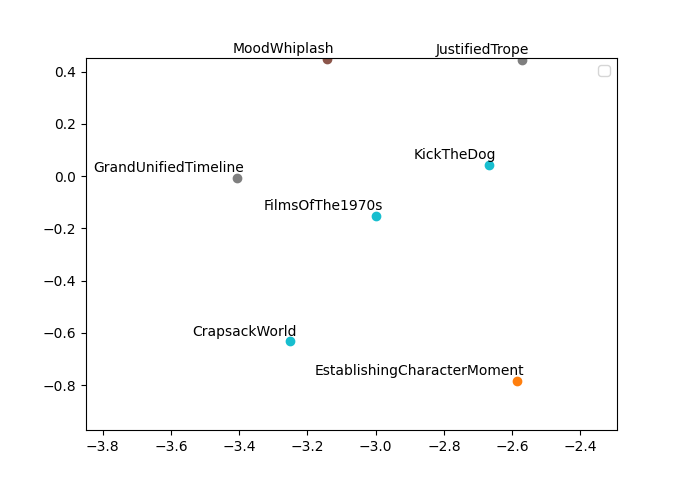
\includegraphics[width=0.85\textwidth,keepaspectratio]{ampliacion_fecha.png}
		\\
		\footnotesize(Ampliación t-SNE)
    \end{center}
\end{frame}

\begin{frame}
	\begin{center}
		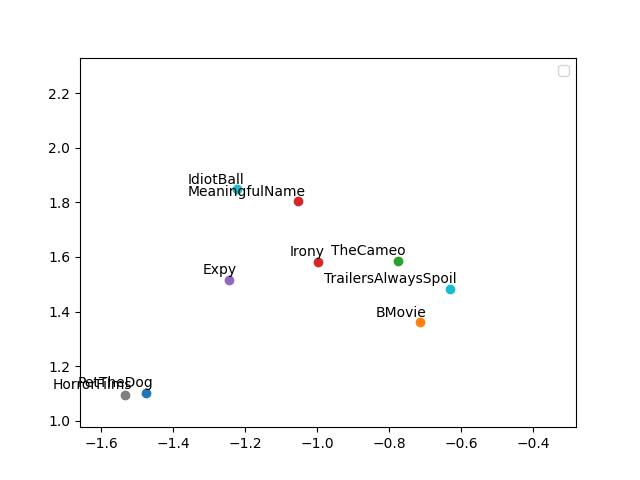
\includegraphics[width=0.85\textwidth,keepaspectratio]{meta.png}
		\\
		\footnotesize(Ampliación t-SNE)
    \end{center}
\end{frame}

\section{Conclusiones y trabajos futuros}

\begin{frame}{Conclusiones}
\begin{itemize}
	\item Se ha creado con éxito una librería extensible para este tipo de investigación.
	\item Se puede extraer cierta información adicional de tropos usando esta técnica,
	pero no parece la más adecuada.
\end{itemize}
\end{frame}

\begin{frame}{Trabajos futuros}
	\begin{itemize}
		\item Investigar formas adicionales de considerar el contexto en tropos.
		\item Añadir etiquetas adicionales al conjunto de datos.
		\item Mejorar la eficiencia del modelo.
		\item Probar modelos alternativos.
	\end{itemize}
\end{frame}

\end{document}